\documentclass{standalone}

\usepackage{tikz}
\usetikzlibrary{angles,quotes}
\usepackage{amsmath,amssymb,amsfonts}

\usepackage{pgfplots}
\usepackage[makeroom]{cancel}
\usetikzlibrary{decorations.markings}
\definecolor{darkgreen}{rgb}{0.0, 0.42, 0.24}
\definecolor{amethyst}{rgb}{0.6, 0.4, 0.8}

\pgfplotsset{compat=newest}
\pgfplotsset{every axis/.append style={
                     tick label style={font=\footnotesize},
                 }}

\begin{document}
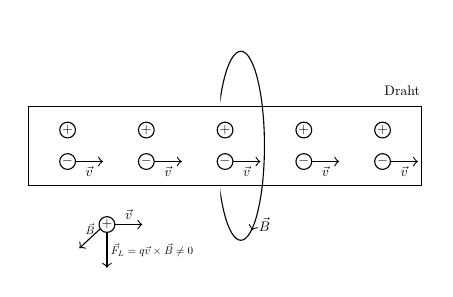
\begin{tikzpicture}
    \draw[draw=black] (0,0) rectangle ++(5,1);
    \draw[](4.75,1.2) node[scale=0.5]{Draht};
    \foreach \a in {0.5, 1.5, ..., 4.5}{
        \draw (\a,0.7) circle [radius=0.1] node[scale=0.5] {$+$};
        \draw (\a,0.3) circle [radius=0.1] node[scale=0.5] {$-$}; 
         \draw[->](\a+0.1,0.3)--(\a+0.45,0.3) node[midway,below,scale=0.5]{$\vec{v}$};
        }   

        \begin{scope}
            \clip (2.439,-1) rectangle ++(2.5,3);
            \draw[decoration={markings, mark=at position 0.8 with {\arrow{<}}},
        postaction={decorate}] (2.7,0.5) ellipse (0.3 and 1.2) ;
        \end{scope}
        \draw[](3,-0.5) node[scale=0.5]{$\vec{B}$};

        \draw (1,-0.5) circle [radius=0.1] node[scale=0.5]{$+$};
        \draw[->](1+0.1,-0.5)--(1+0.45,-0.5) node[midway,above,scale=0.5]{$\vec{v}$};
        \draw[->](1,-0.6)--(1,-0.6-0.45) node[midway,right,scale=0.4]{$\vec{F}_L=q\vec{v}\times\vec{B}\neq0$};
        \draw[->](0.92,-0.55)--(0.65,-0.8) node[midway,above,scale=0.4]{$\vec{B}$};
\end{tikzpicture}
\end{document}